\section{Методы решения нелинейных уравнений и систем нелинейных уравнений}

\subsection{Постановка задачи}
2.1. Реализовать методы простой итерации и Ньютона решения нелинейных уравнений в виде программ, задавая в качестве входных данных точность вычислений. С использованием разработанного программного обеспечения найти положительный корень нелинейного уравнения (начальное приближение определить графически). Проанализировать зависимость погрешности вычислений от количества итераций. 

{\bfseries Вариант:} 19
    \begin{equation}
        x^4 - 2x - 1 = 0
    \end{equation}
\pagebreak

\subsection{Результаты работы}
\begin{figure}[h!]
\centering
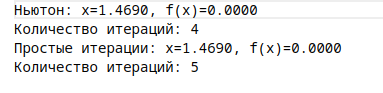
\includegraphics[width=.5\textwidth]{lab2.1}
\caption{Вывод в консоли}
\end{figure}


\subsection{Исходный код}
\lstinputlisting[title=\texttt{Lab2.1.cpp}]{../stud/saifullin/task2.1/Lab2.1.cpp}
\pagebreak

